\section{Symmetry: The Weak Interaction}
\subsection{Symmetry Breaking}
\begin{itemize}
    \item The breaking of gauge symmetry by the BEH mechanism is what gives mass. 
    \item Breaking of isospin symmetry by the $u$ and $d$ quark mass difference and electric charge difference. 
\end{itemize}
\subsubsection{Weak Parity Violation}
\paragraph{Cobalt Decay \cref{fig: cobalt_symmetry_breaking}}
Polarized $^{60}$Co decays into $^{60}$Ni, an electron neutrino and an electron. For parity to be conserved we would have\vbox{:}
\begin{wrapfigure}[8]{r}{0.45\textwidth}
\centering
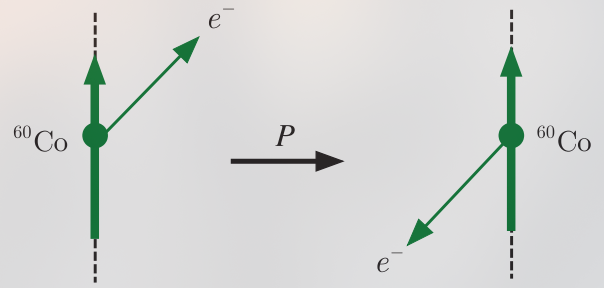
\includegraphics[width = .4\textwidth]{cobalt_symmetry_breaking.png}
\caption{Parity affecting the decay of a Cobalt atom.}
\label{fig: cobalt_symmetry_breaking}
\end{wrapfigure}
\begin{align}
  \vec{r} &→ -\vec{r} \\
  \vec{p} &→ -\vec{p} \\
  \vec{r} × \vec{p} &→ \vec{r} × \vec{p} \\
  \vec{J}, \vec{S}, \vec{L} &→ \vec{J}, \vec{S}, \vec{L}
\end{align}
This was experimentally shown to not be the case, as the above implies that there should be as many particles scattered at angle $θ$, as angel $π - θ$. 



\paragraph{Muon Decay \cref{fig: muon_symmetry_breaking}}
\begin{wrapfigure}[6]{r}{0.45\textwidth}
    \centering
    \vspace{-5mm}
    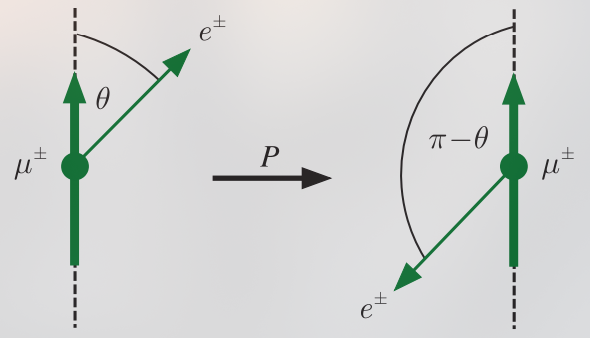
\includegraphics[width = .4\textwidth]{muon_symmetry_breaking.png}
    \caption{Parity affecting the decay of a muon.}
    \label{fig: muon_symmetry_breaking}
\end{wrapfigure}
\begin{itemize}
    \item We see parity not being conserved as $θ$ and $π - θ$ are not equal.
    \item We also see that $C$-parity is not conserved. 
    \item The product $CP$ is conserved, making the lifetime of $ℏ/Γ_{+} = ℏ/Γ_{-}$.     
\end{itemize}

\subsection{CP Conservation}
\begin{itemize}
  \item $CP$ is conserved when both $C$ and $P$ are conserved separately in the strong and electromagnetic interactions.
  \item $CP$ is conserved in nearly all weak interactions. 
\end{itemize}

\subsection{Chirality and Helicity}
\begin{itemize}
  \item Helicity is when the spin is in the same or opposite direction as the momentum. This can change for massless particles, as you can theoretically move faster than then, and from your perspective, the spin would be in the opposite direction.
  \item Chirality is harder to define, and represent an intrinsic property of a particle, as opposed to helicity being an observable which is relative. One can be left- or right-chiral. One can only change it by viewing it in a mirror image, as you flip it's spin, but not momentum. If you boost your velocity to be higher than a particle, it will change it's helicity, but not it's chirality.
  \item The weak interaction only couples to left-chiral particles and right-handed anti-particles, but both left and right-handed particles. 
\end{itemize}
\subsubsection{Right- and Left-Handedness \cref{fig: left_vs_right_handedness}}
\begin{figure}[h!]
\centering
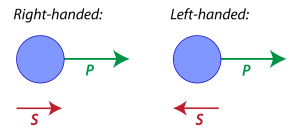
\includegraphics[width = \textwidth]{left_vs_right_handedness.png}
\caption{Figure showing difference between left- and right-handed particles. A no-handed particle would have spin-0, or $J_z = 0$, meaning perpendicular to the direction of motion.}
\label{fig: left_vs_right_handedness}
\end{figure}

\subsubsection{The Weak Interaction}  
\begin{itemize}
  \item Eigenstates of the chirality takes part of the weak interaction as a conserved charge. 
  \item For massless particles, the helicity is the same as the chirality.
  \begin{equation}
    h ≡ \vec{J} ⋅  \frac{\vec{p}}{\left|\vec{p}\right|}
  \end{equation} 
  \item The helicity state's magnitude is the same as it's spin magnitude. The sign is positive for right-handed particles and negative for left-handed particles.
  \item Photons have only helicity $±1$, as they are massless.
  \item Massive bosons have helicity states $±1$ and $0$.
\end{itemize}


\subsubsection{Electron-Electron Scattering \cref{fig: electron_electron_parity}}
\begin{itemize}
  \item \textbf{Upper Left:} The initial beam is right-handed. 
  \item \textbf{Upper Right:} The beam becomes left-handed after the parity transformation. This is because both, momentum and position is flipped, but the spin is not.
  \item \textbf{Lower Right:} Changing our perspective by flipping $180^∘$ along the $y$-axis. 
  \item \textbf{Lower Left:} Changing our perspective by flipping $180^∘$ along the $x$-axis. We now have the original state, but with left-handed particles. For parity to be conserved, the cross section $σ_{R}$ and $σ_{L}$, should be the same, and they are. 
\end{itemize}
\begin{figure}[ht!]
\centering
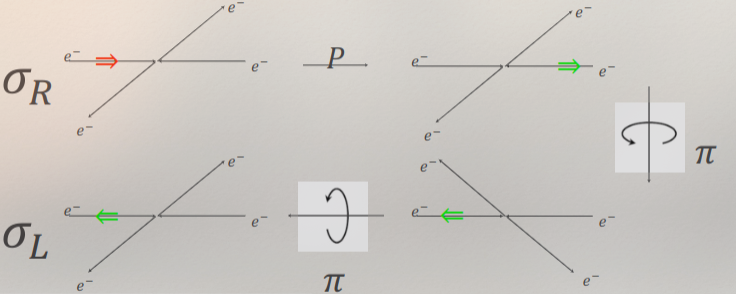
\includegraphics[width = \textwidth]{electron_electron_parity.png}
\caption{Electron-electron scattering viewed from with after parity transformation and change of perspective.}
\label{fig: electron_electron_parity}
\end{figure}

\subsection{V - A Interaction}
\begin{itemize}
  \item $V$ is a vector interaction, like $\vec{r}$ changing sign under parity.
  \item $A$ is an axial vector interaction, like $\vec{L} ≡ \vec{r} × \vec{p}$ changing sign under parity.
  \item Both $\left|\mathcal{M}\right|^2 \propto \left|V^2\right|$ or $\left|A\right|^2$, would be parity conserving, but interference terms $\left|\mathcal{M}\right|^2 \propto \left|V - A\right|^2$ violates it. 
  \item $W^{±}$ couples to the $V-A$ weak current 
  \item $Z^{0}$ couples to mixtures of $V$ and $A$, depending on the 3rd component of weak isospin, electric charge and $\sin^2 θ_{W}$
\end{itemize}

\subsection{Neutral Kaon Oscillation}
\begin{itemize}
  \item The Kaon $d \bar{s}$, can oscillate between $K^{0}$ and $\bar{K}^{0}$. This is a $\left|ΔS\right| = 2$ transition allowed by second-order weak interactions. 
  \item It is second order because there are two decays, as seen in \cref{fig: kaon_oscillation}, and comes about because the decay products live long enough. 
\end{itemize}
\begin{figure}[h!]
\centering
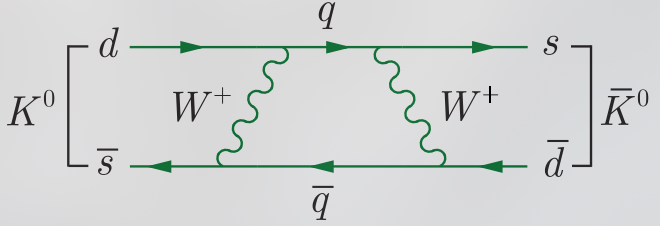
\includegraphics[width = \textwidth]{kaon_oscillation.png}
\caption{Feynman diagram showing the oscillation of a neutral Kaon. $q$ can be any up-type quark, and $\bar{q}$ any up-type anti-quark.}
\label{fig: kaon_oscillation}
\end{figure}

